\documentclass[xetex,mathserif,serif]{beamer}
\usepackage{polyglossia}
\setdefaultlanguage[babelshorthands=true]{russian}
\usepackage{minted}
\usepackage{tabu}
\usepackage{moresize}

\useoutertheme{infolines}

\usepackage{fontspec}
\setmainfont{FreeSans}
\newfontfamily{\russianfonttt}{FreeSans}

\definecolor{links}{HTML}{2A1B81}
\hypersetup{colorlinks,linkcolor=,urlcolor=links}

\setbeamertemplate{blocks}[rounded][shadow=false]

\setbeamercolor*{block title alerted}{fg=red!50!black,bg=red!20}
\setbeamercolor*{block body alerted}{fg=black,bg=red!10}

\tabulinesep=1.2mm

\title{Об учебных практиках}
\author[Юрий Литвинов]{Юрий Литвинов\\\small{\textcolor{gray}{y.litvinov@spbu.ru}}}
\date{30.11.2021}

\newcommand{\attribution}[1] {
\vspace{-5mm}\begin{flushright}\begin{scriptsize}\textcolor{gray}{\textcopyright\, #1}\end{scriptsize}\end{flushright}
}

\begin{document}

    \frame{\titlepage}

    \section{Общие требования}

    \begin{frame}
        \frametitle{Зачёт по учебной практике}
        \begin{itemize}
            \item Отчёт по практике
            \begin{itemize}
                \item Порядка 5-7 содержательных страниц
                \item У каждого свой, даже если работа групповая
                \item Переиспользование фрагментов текста недопустимо
                \item Сдать до 15 декабря
            \end{itemize}
            \item Отзыв руководителя
            \begin{itemize}
                \item В виде скана с подписью
            \end{itemize}
            \item Доклад с презентацией
            \begin{itemize}
                \item На 5-7 минут, порядка 10 слайдов
                \item Может быть одним на весь проект
            \end{itemize}
        \end{itemize}
    \end{frame}

    \section{Отчёт}

    \begin{frame}
        \frametitle{Про тексты курсовых}
        \framesubtitle{Структура отчёта}
        \begin{itemize}
            \item Титульный лист (см. \url{https://oops.math.spbu.ru/SE/YearlyProjects/vesna-2020/practices})
            \item Оглавление
            \item Введение в предметную область, постановка задачи
            \item Обзор литературы и существующих решений
            \item Описание предлагаемого решения, сравнение с существующими
            \item Заключение
            \item Список источников (ГОСТ Р 7.0.5--2008)
            \item Приложения (если есть)
        \end{itemize}
    \end{frame}

    \begin{frame}
        \frametitle{Введение}
        \begin{columns}
            \begin{column}{0.6\textwidth}
                \begin{itemize}
                    \item Известная информация, ``Background''
                    \item Неизвестная информация, ``Gap''
                    \begin{itemize}
                        \item Актуальность темы
                        \item Практическая значимость
                    \end{itemize}
                    \item Цель работы, ``Гипотеза'' 
                    \item Задачи, необходимые для достижения цели, ``Подход''
                \end{itemize}
            \end{column}
            \begin{column}{0.4\textwidth}
                \begin{center}
                    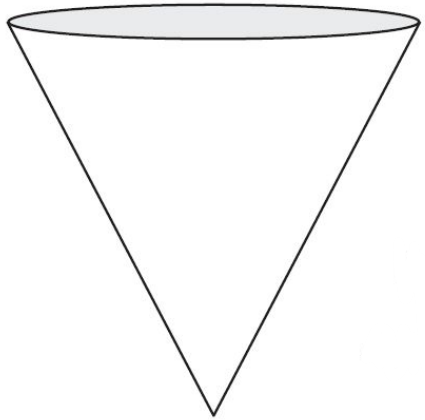
\includegraphics[width=\textwidth]{introductionCone.png}
                \end{center}
            \end{column}
        \end{columns}
    \end{frame}

    \begin{frame}
        \frametitle{Постановка задачи}
        \begin{itemize}
            \item Цель работы --- одно предложение
            \begin{itemize}
                \item ``Целью работы является ...''
            \end{itemize}
            \item Задачи --- 3-5 пунктов в виде списка
            \begin{itemize}
                \item Выполнить обзор существующих решений
                \item Разработать алгоритм/архитектуру
                \item Реализовать
                \item Провести апробацию/тестирование/эксперименты
            \end{itemize}
            \item Задачи должны быть специфичны
        \end{itemize}
    \end{frame}

    \begin{frame}
        \frametitle{Обзор}
        \begin{itemize}
            \item Обзор существующих решений
            \begin{itemize}
                \item Цель и фокус обзора
                \item Критерии сравнения
                \item Выводы
            \end{itemize}
            \item Обзор используемых чужих результатов
            \begin{itemize}
                \item Всё, написанное и придуманное не вами --- в обзор
            \end{itemize}
            \item Должен соотноситься с темой и с фокусом работы
        \end{itemize}
    \end{frame}

    \begin{frame}
        \frametitle{Описание решения}
        \begin{itemize}
            \item Желательно, чтобы разделы отвечали решению задачи из списка задач во введении
            \item Аргументированное обоснование принятых решений и отказа от альтернатив
            \item Описание программной реализации, архитектура
            \item Эксперименты и апробация
            \item Выводы и обсуждение
        \end{itemize}
    \end{frame}

    \begin{frame}
        \frametitle{Заключение}
        \begin{itemize}
            \item Перечисление результатов, выносимых на защиту
            \item Должно быть согласовано с постановкой задачи (вплоть до полного её повторения)
            \item Должно быть согласовано с текстом
            \item Никаких результатов из ниоткуда
        \end{itemize}
    \end{frame}

    \begin{frame}
        \frametitle{Общие замечания}
        \begin{itemize}
            \item Каждый рисунок --- пронумерован и подписан, есть ссылка из текста
            \item На каждый элемент списка литературы ссылка из текста
            \item Никакого плагиата!
            \item Полезно сначала написать план
            \item \url{https://papeeria.com/}, \url{https://www.overleaf.com/}
        \end{itemize}
    \end{frame}

    \section{Презентация}

    \begin{frame}
        \frametitle{Презентация}
        \begin{itemize}
            \item Доклад на 5-7 минут
            \item Возможна одна презентация на несколько человек, но у каждого должен быть свой слайд с результатами
            \item Чеклист по презентации: \url{https://docs.google.com/spreadsheets/d/1LvHveX6TdbzexuACcqGPeHIEph6cm4Hd0arCRQBqODw}
            \item Презентации прошлых лет: \url{https://oops.math.spbu.ru/SE/YearlyProjects/vesna-2020/practices}
        \end{itemize}
    \end{frame}

    \begin{frame}
        \frametitle{Структура презентации}
        \begin{itemize}
            \item Титульный слайд 
            \begin{itemize}
                \item Тема, автор, научник (учёная степень если есть, должность)
            \end{itemize}
            \item Введение
            \begin{itemize}
                \item Краткий рассказ про предметную область
                \item Обосновать актуальность задачи
            \end{itemize}
            \item Постановка задачи (обязательно!)
            \begin{itemize}
                \item ``Целью работы является...''
                \item Список из 3-5 задач, которые надо было решить для достижения цели
                \item ``Сделать обзор'' (чего?), ``Разработать архитектуру'', ``Реализовать'', ``Провести эксперименты''...
            \end{itemize}
        \end{itemize}
    \end{frame}

    \begin{frame}
        \frametitle{Структура презентации (2)}
        \begin{itemize}
            \item Обзор
            \begin{itemize}
                \item Существующие решения
                \item Используемые технологии
                \item Всё, что делали не вы, но что нужно для понимания работы
            \end{itemize}
            \item Описание реализации
            \begin{itemize}
                \item Архитектура (UML-диаграммы приветствуются)
                \item Особенности реализации (то, над чем пришлось подумать)
            \end{itemize}
            \item Эксперименты
            \begin{itemize}
                \item Численные измерения (нужен матстат --- матожидание, дисперсия)
                \item Подписи к осям
                \item Примеры использования
                \item Сравнение с существующими аналогами, выводы
            \end{itemize}
        \end{itemize}
    \end{frame}

    \begin{frame}
        \frametitle{Структура презентации (3)}
        \begin{itemize}
            \item Результаты
            \begin{itemize}
                \item Список того, что выносится на защиту
                \item Должно соответствовать списку задач (лучше --- полностью повторять, с заменой ``сделать'' на ``сделано'')
                \item Всё, что перечислено в результатах, должно быть отражено ранее на слайдах
                \item Не очень приветствуются неотчуждаемые результаты (типа ``изучил'')
                \item Должно быть последним слайдом
            \end{itemize}
        \end{itemize}
    \end{frame}

\end{document}
